% ===========================================================================
%
%		FEDERICO II THESIS TEMPLATE - ENGLISH
%  					* an example of Chapter 1: information about the discussion of the thesis
%	 
% 		AUTHOR:  		Antonio Esposito (antonio.esposito103@studenti.unina.it)
%		LAST UPDATED:	2017/06/20
%
% ===========================================================================

\chapter{Modello di Dominio}

%%%%% ===============================================================================
%\section{Classi, oggetti e relazioni di analisi}
%Qua vanno messi i class diagram
%%%%% ===============================================================================
\section{Diagrammi di sequenza di analisi}
Si riportano di seguito i diagrammi di sequenza di analisi dei casi d'uso.
\includepdf[pages={1-6}]{SequenceAnalisi/diagrammi.pdf}

\pagebreak
%%%%% ===============================================================================
\section{Diagrammi di stato di attività}
Sono riportati di seguito i diagrammi di stato di alcuni casi d'uso.
\begin{figure}[h!]
    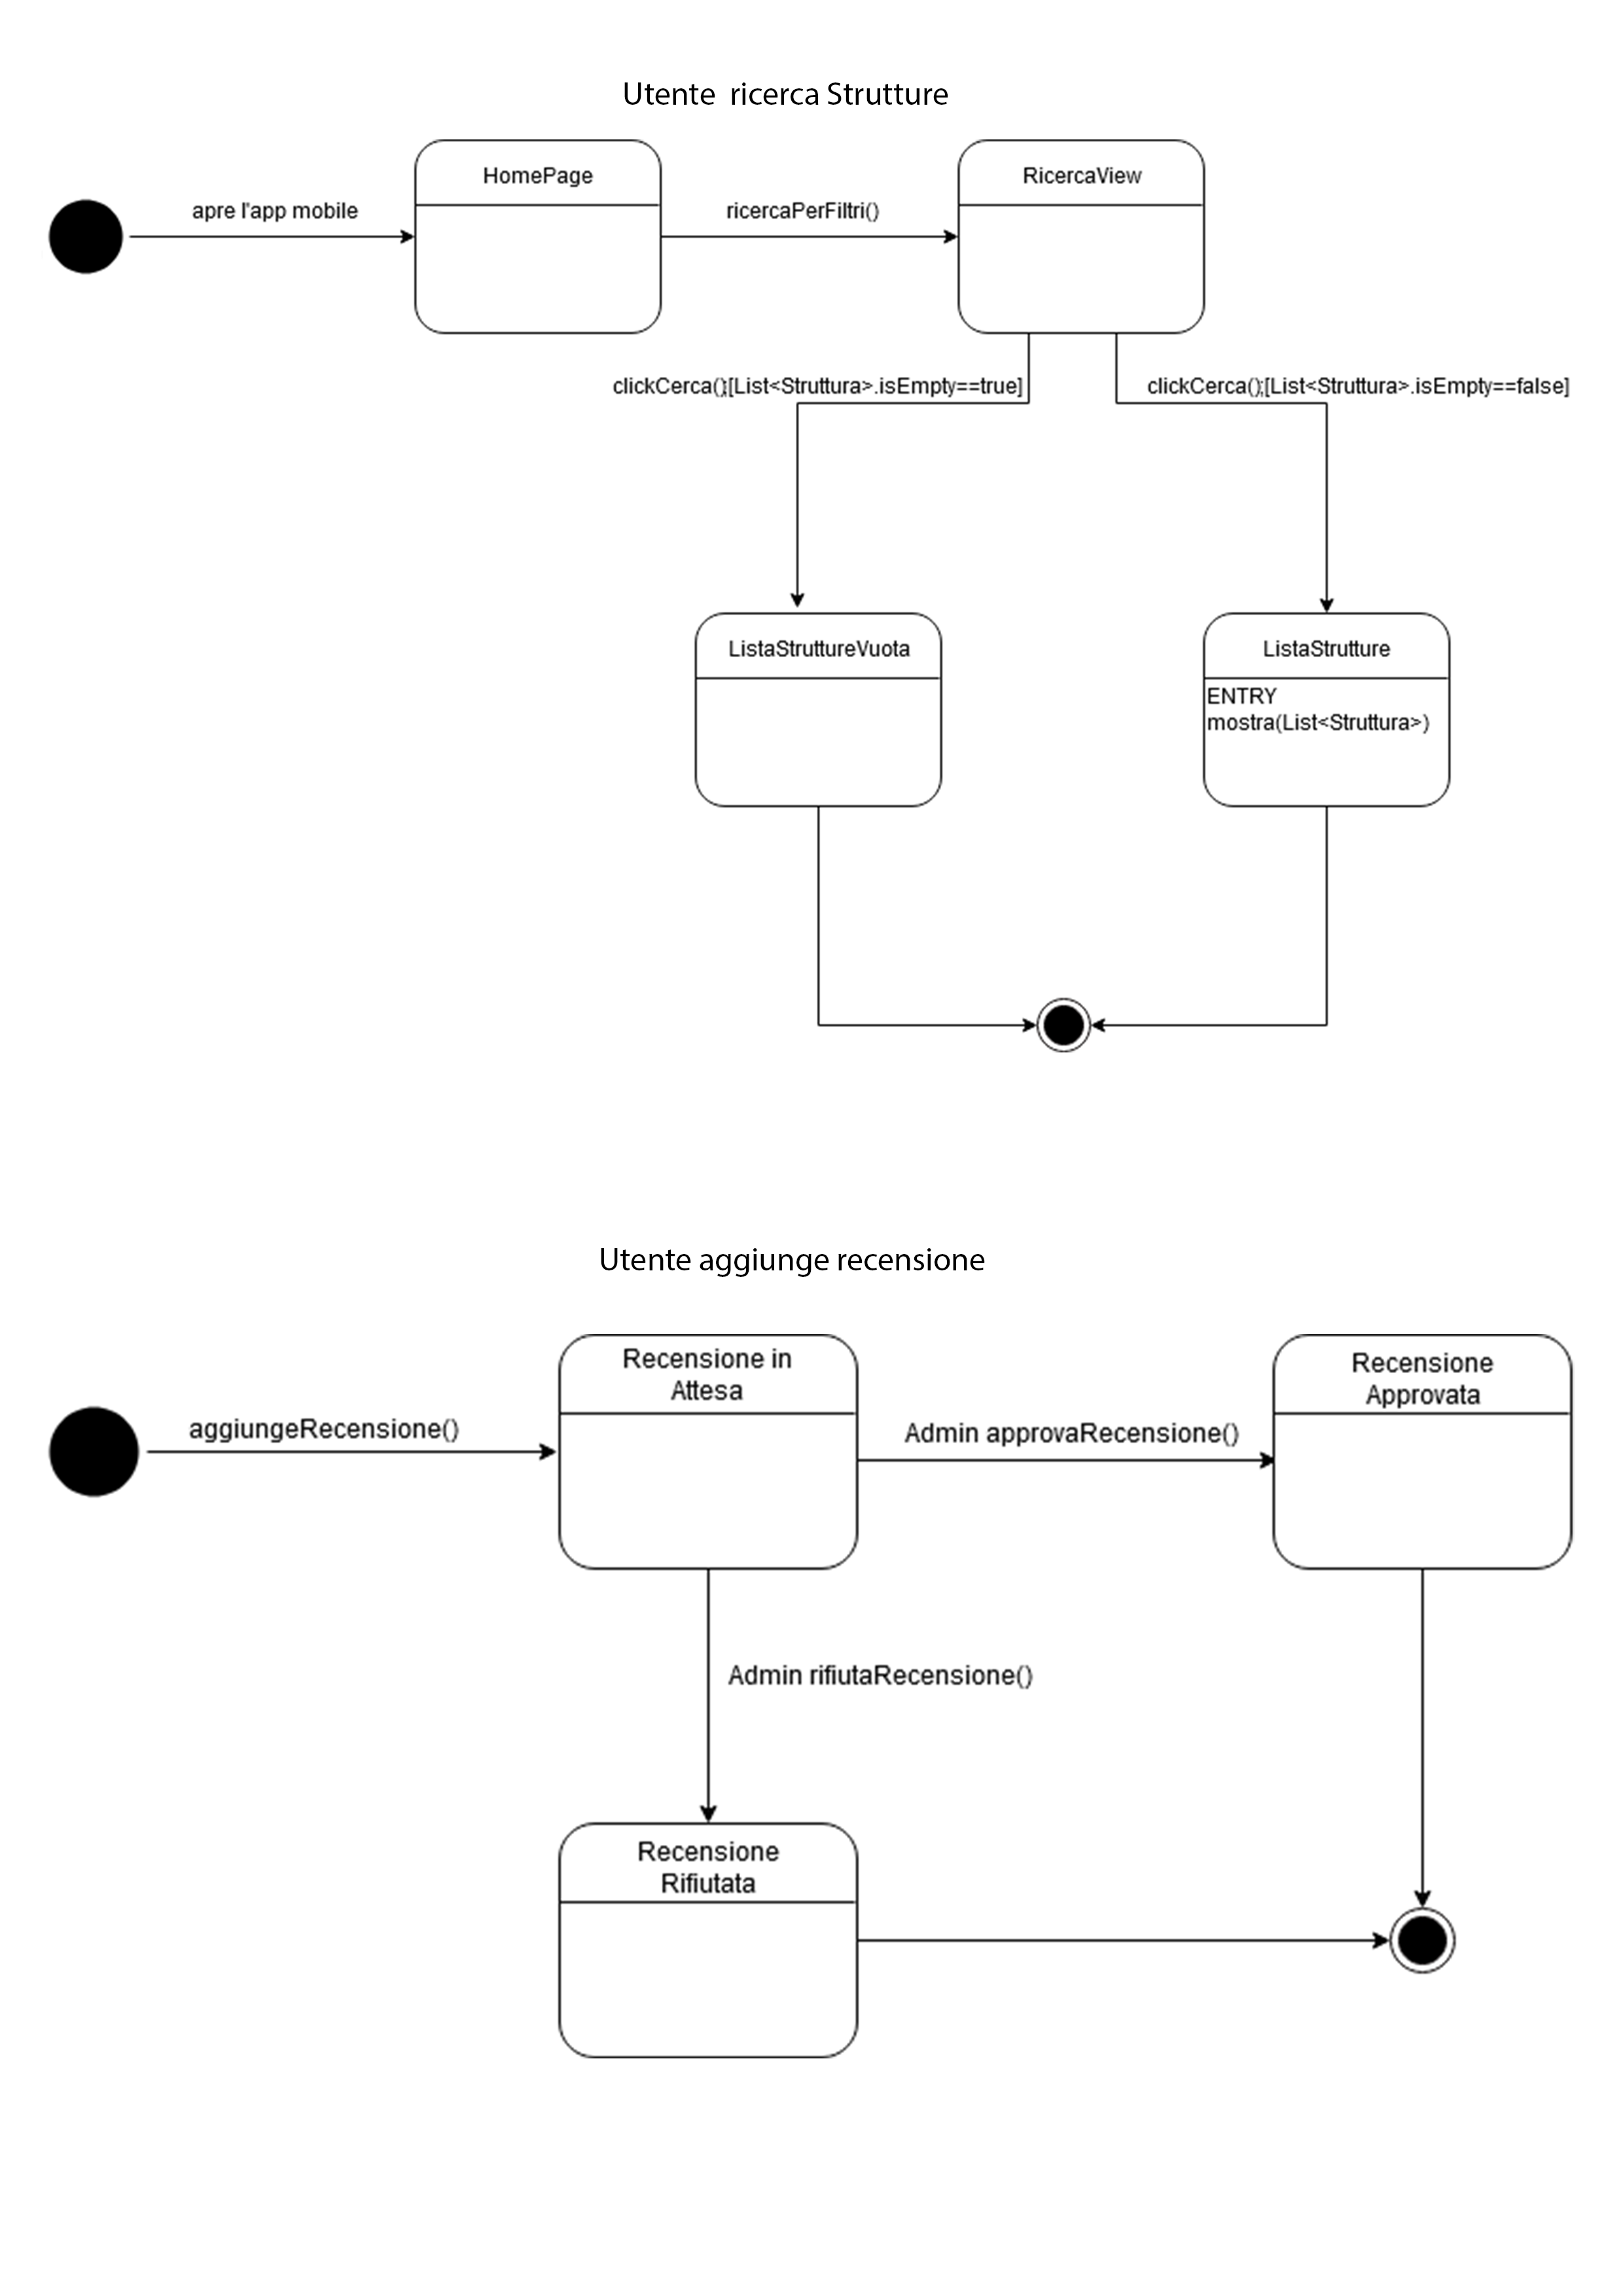
\includegraphics[width=\textwidth]{SequenceAnalisi/7.png}
\end{figure}
\begin{figure}[h!]
    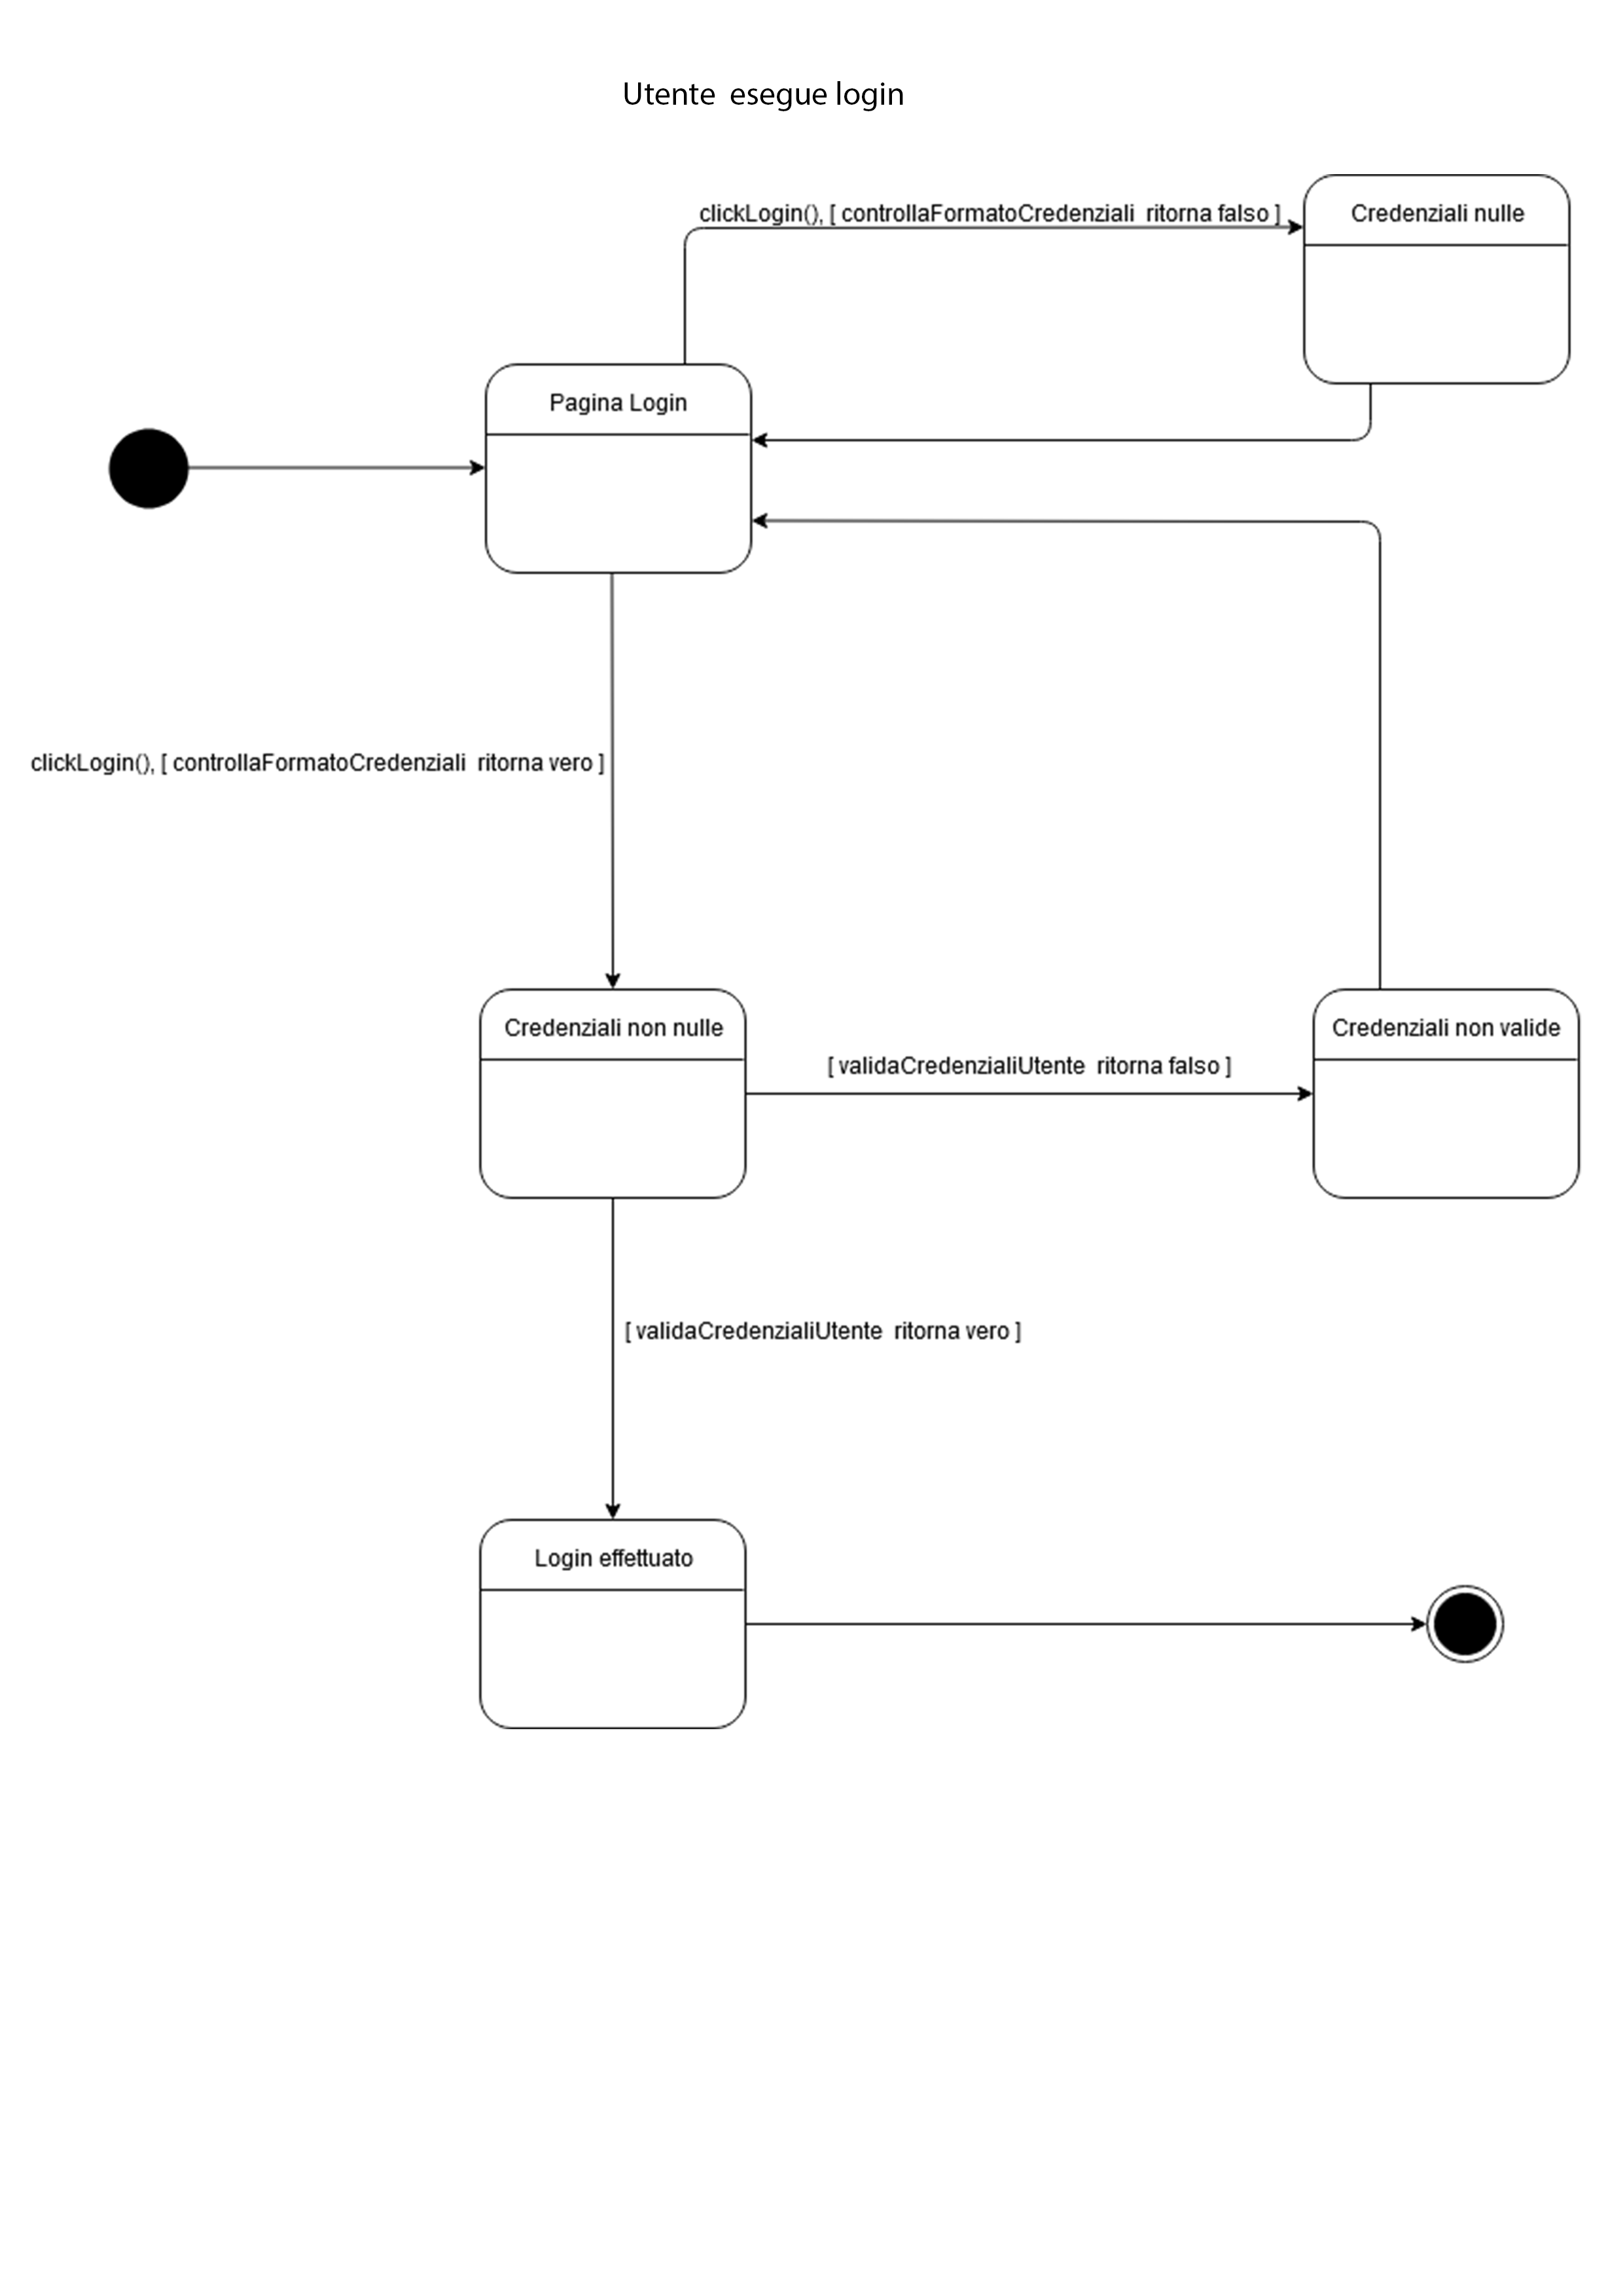
\includegraphics[width=\textwidth]{SequenceAnalisi/8.png}
\end{figure}
\pagebreak
%%%%% ===============================================================================
\section{Diagrammi di attività}
Sono riportati di seguito i diagrammi di attività di alcuni casi d'uso.
\begin{figure}[h!]
    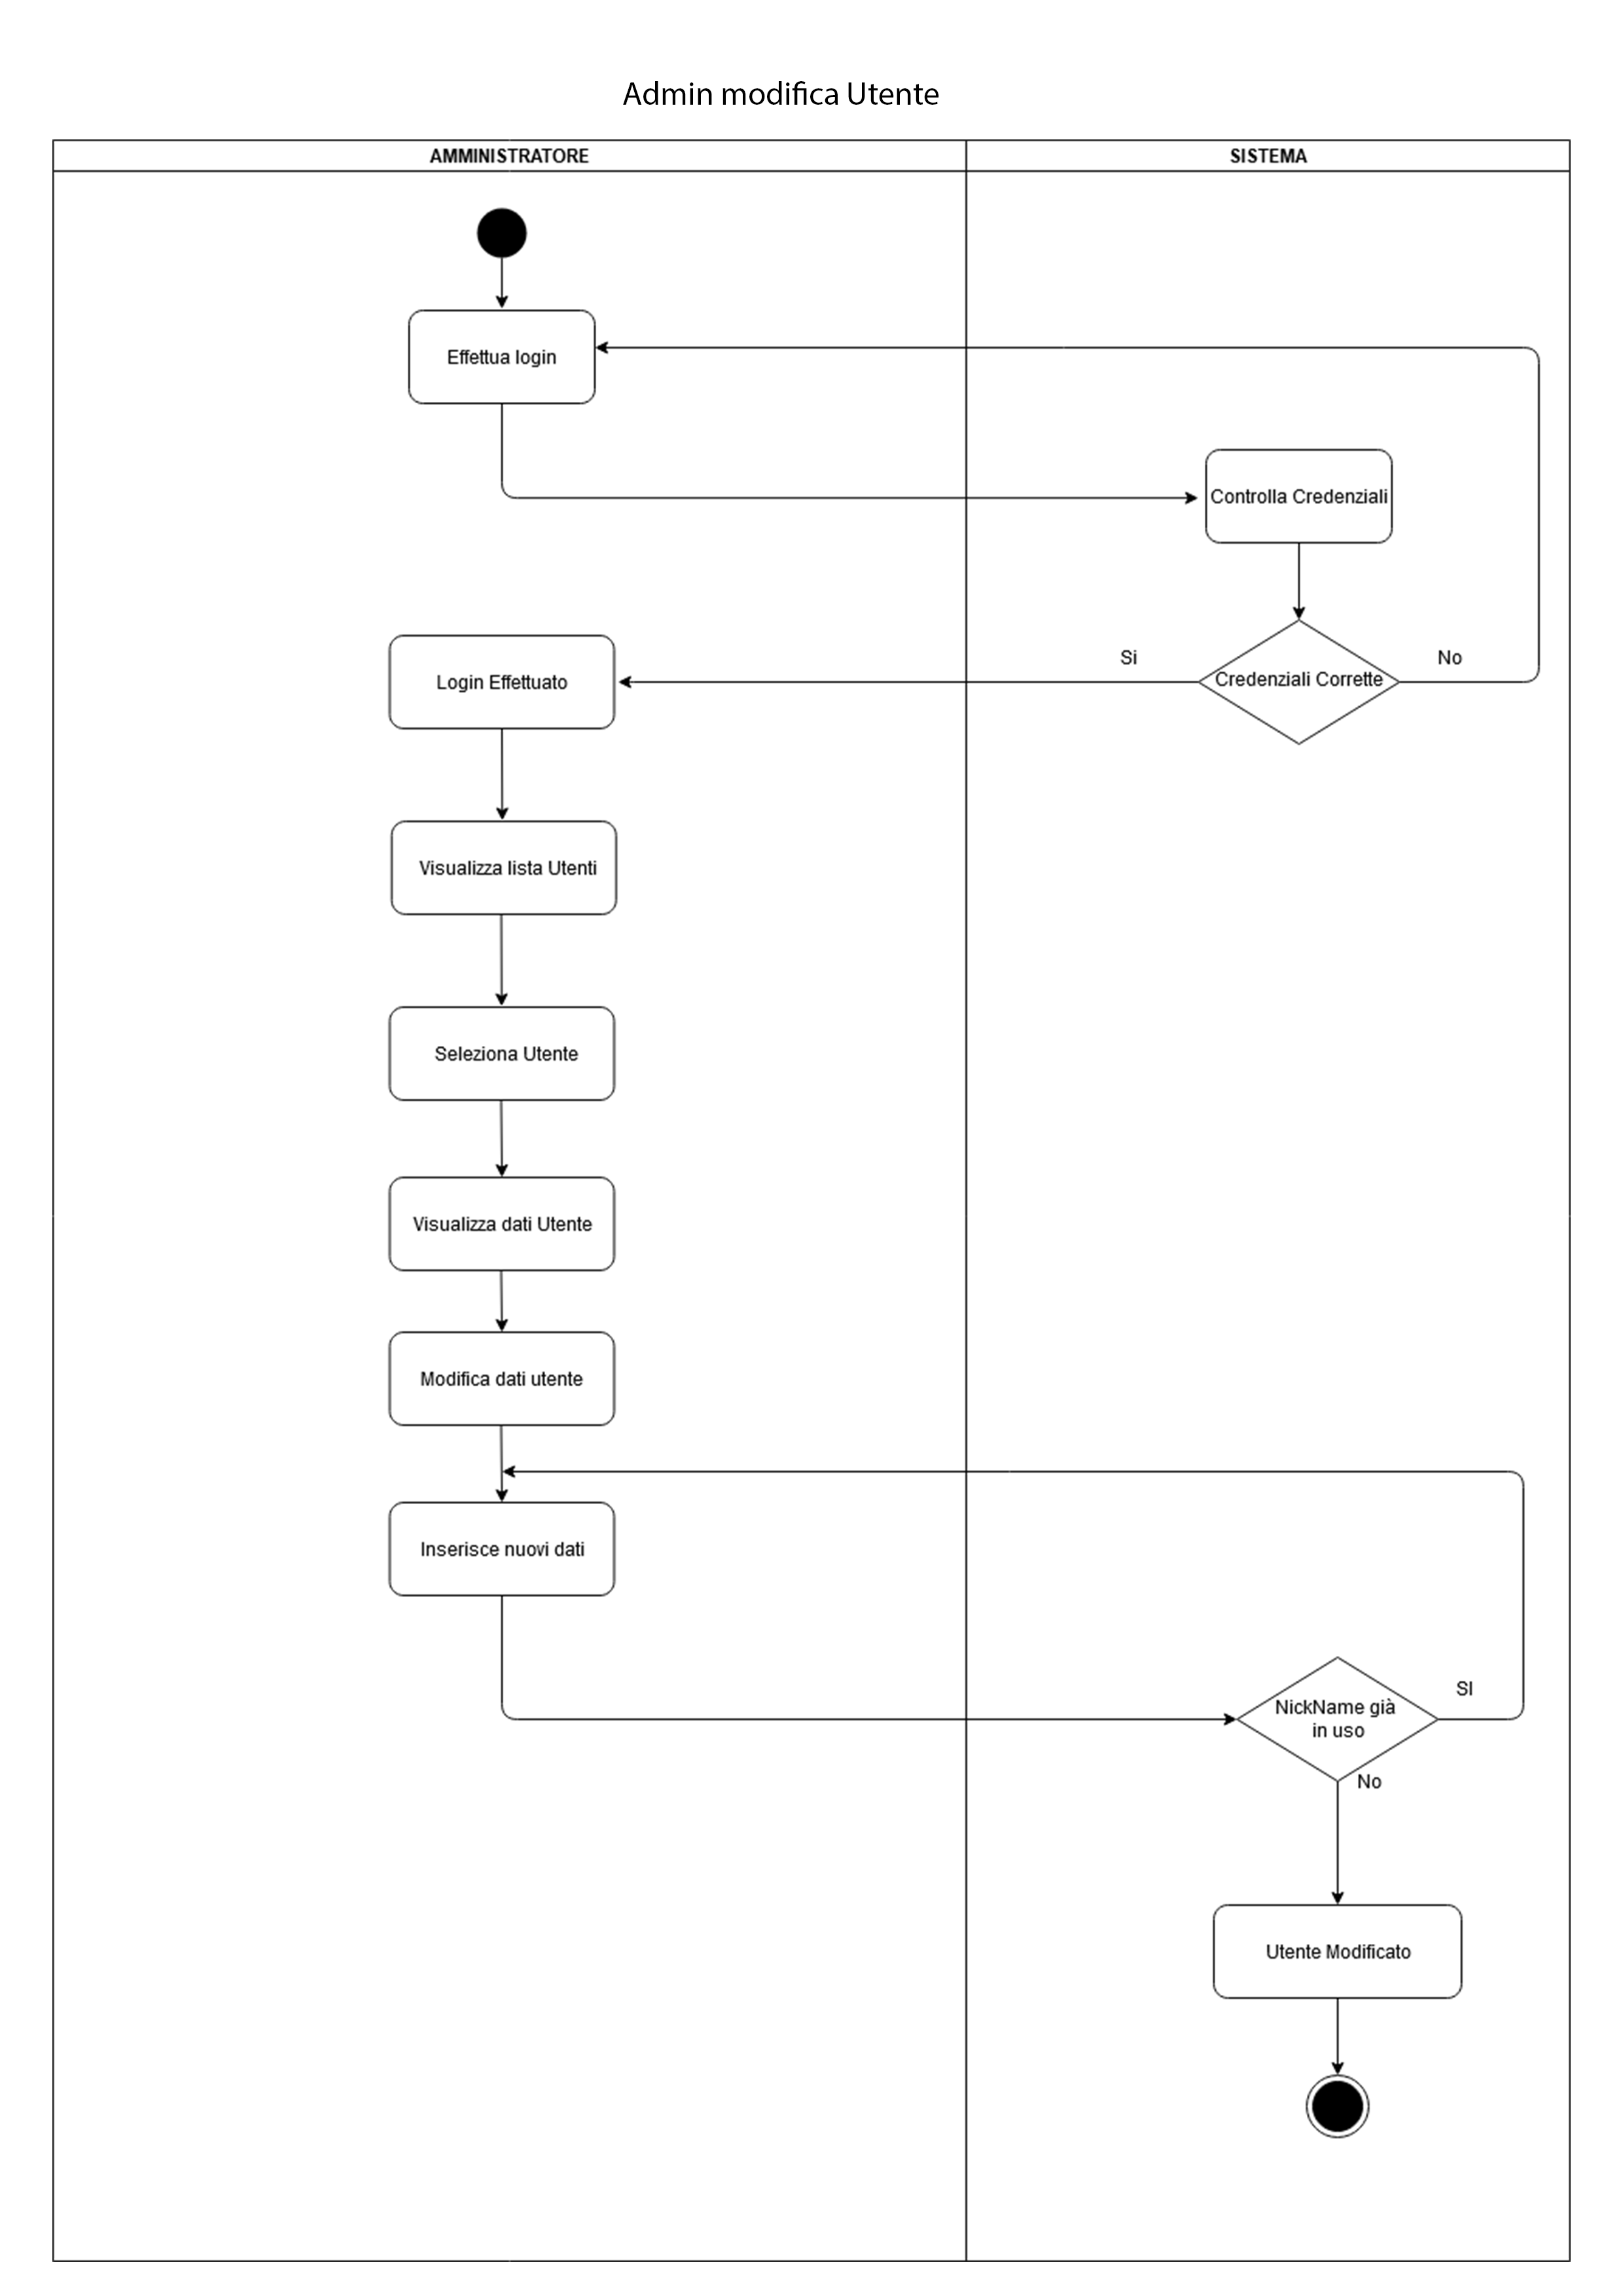
\includegraphics[width=\textwidth]{SequenceAnalisi/9.png}
\end{figure}
\begin{figure}[h!]
    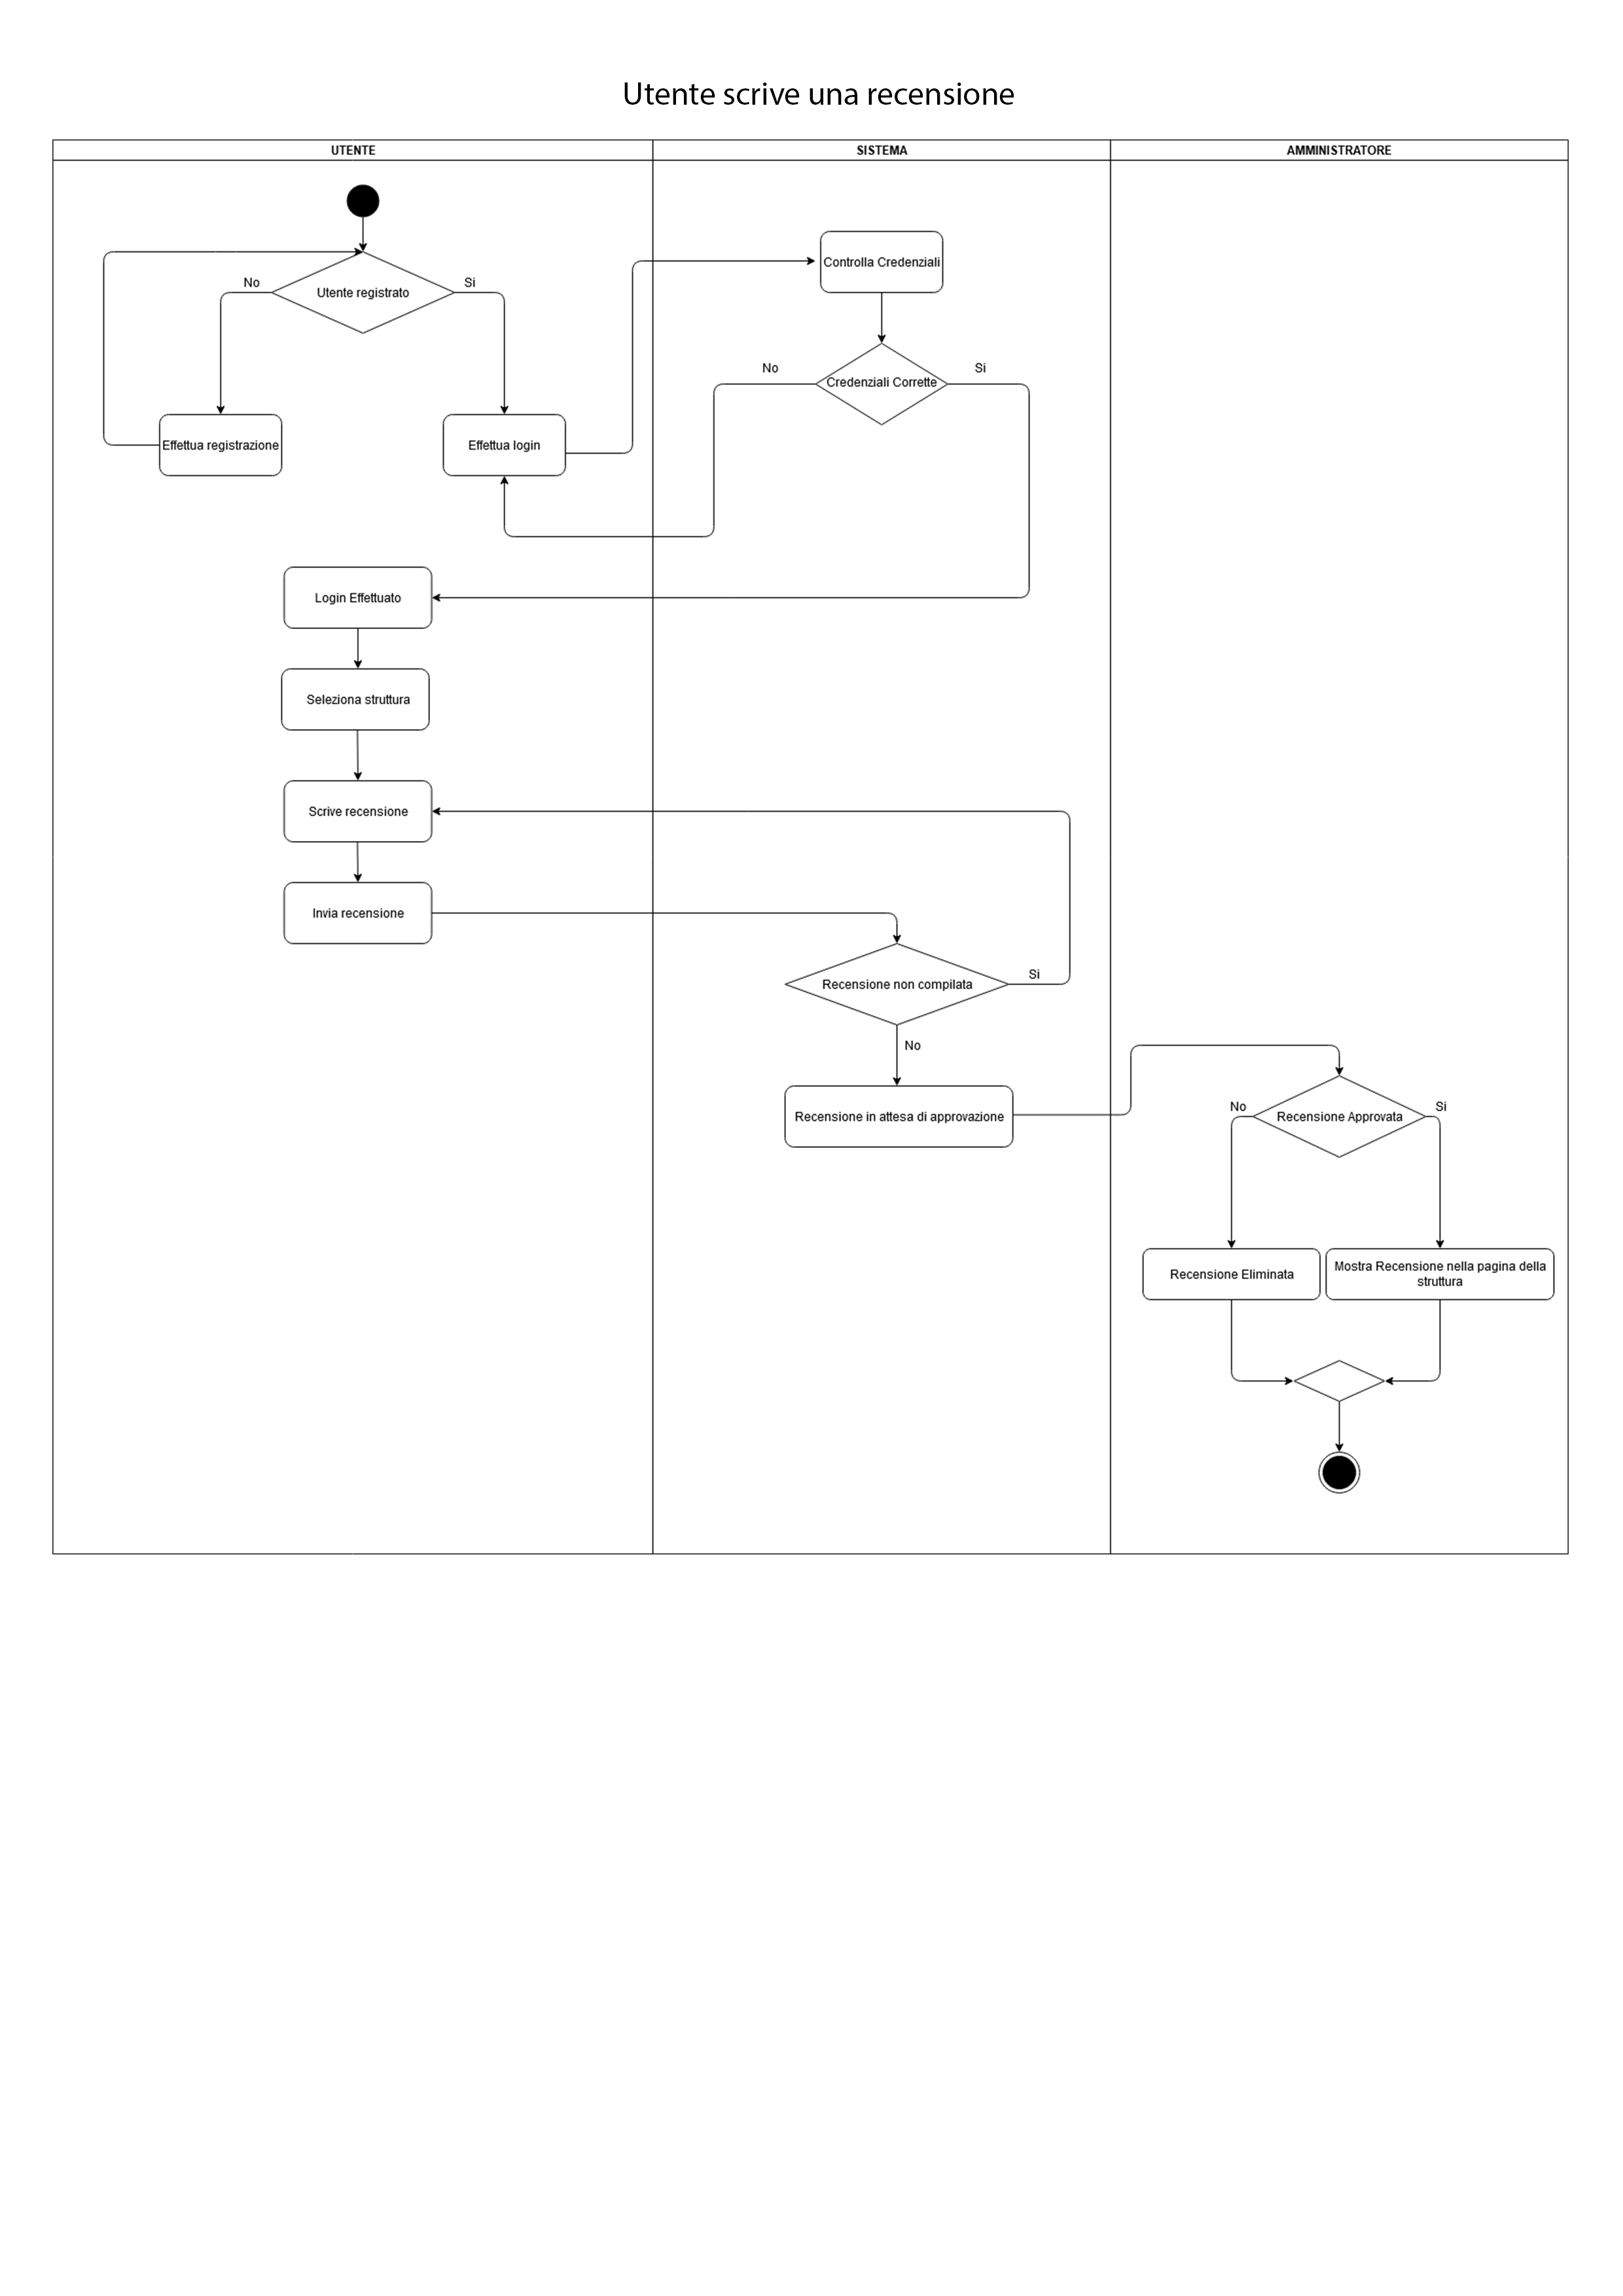
\includegraphics[width=\textwidth]{SequenceAnalisi/10.png}
\end{figure}
\begin{figure}[h!]
    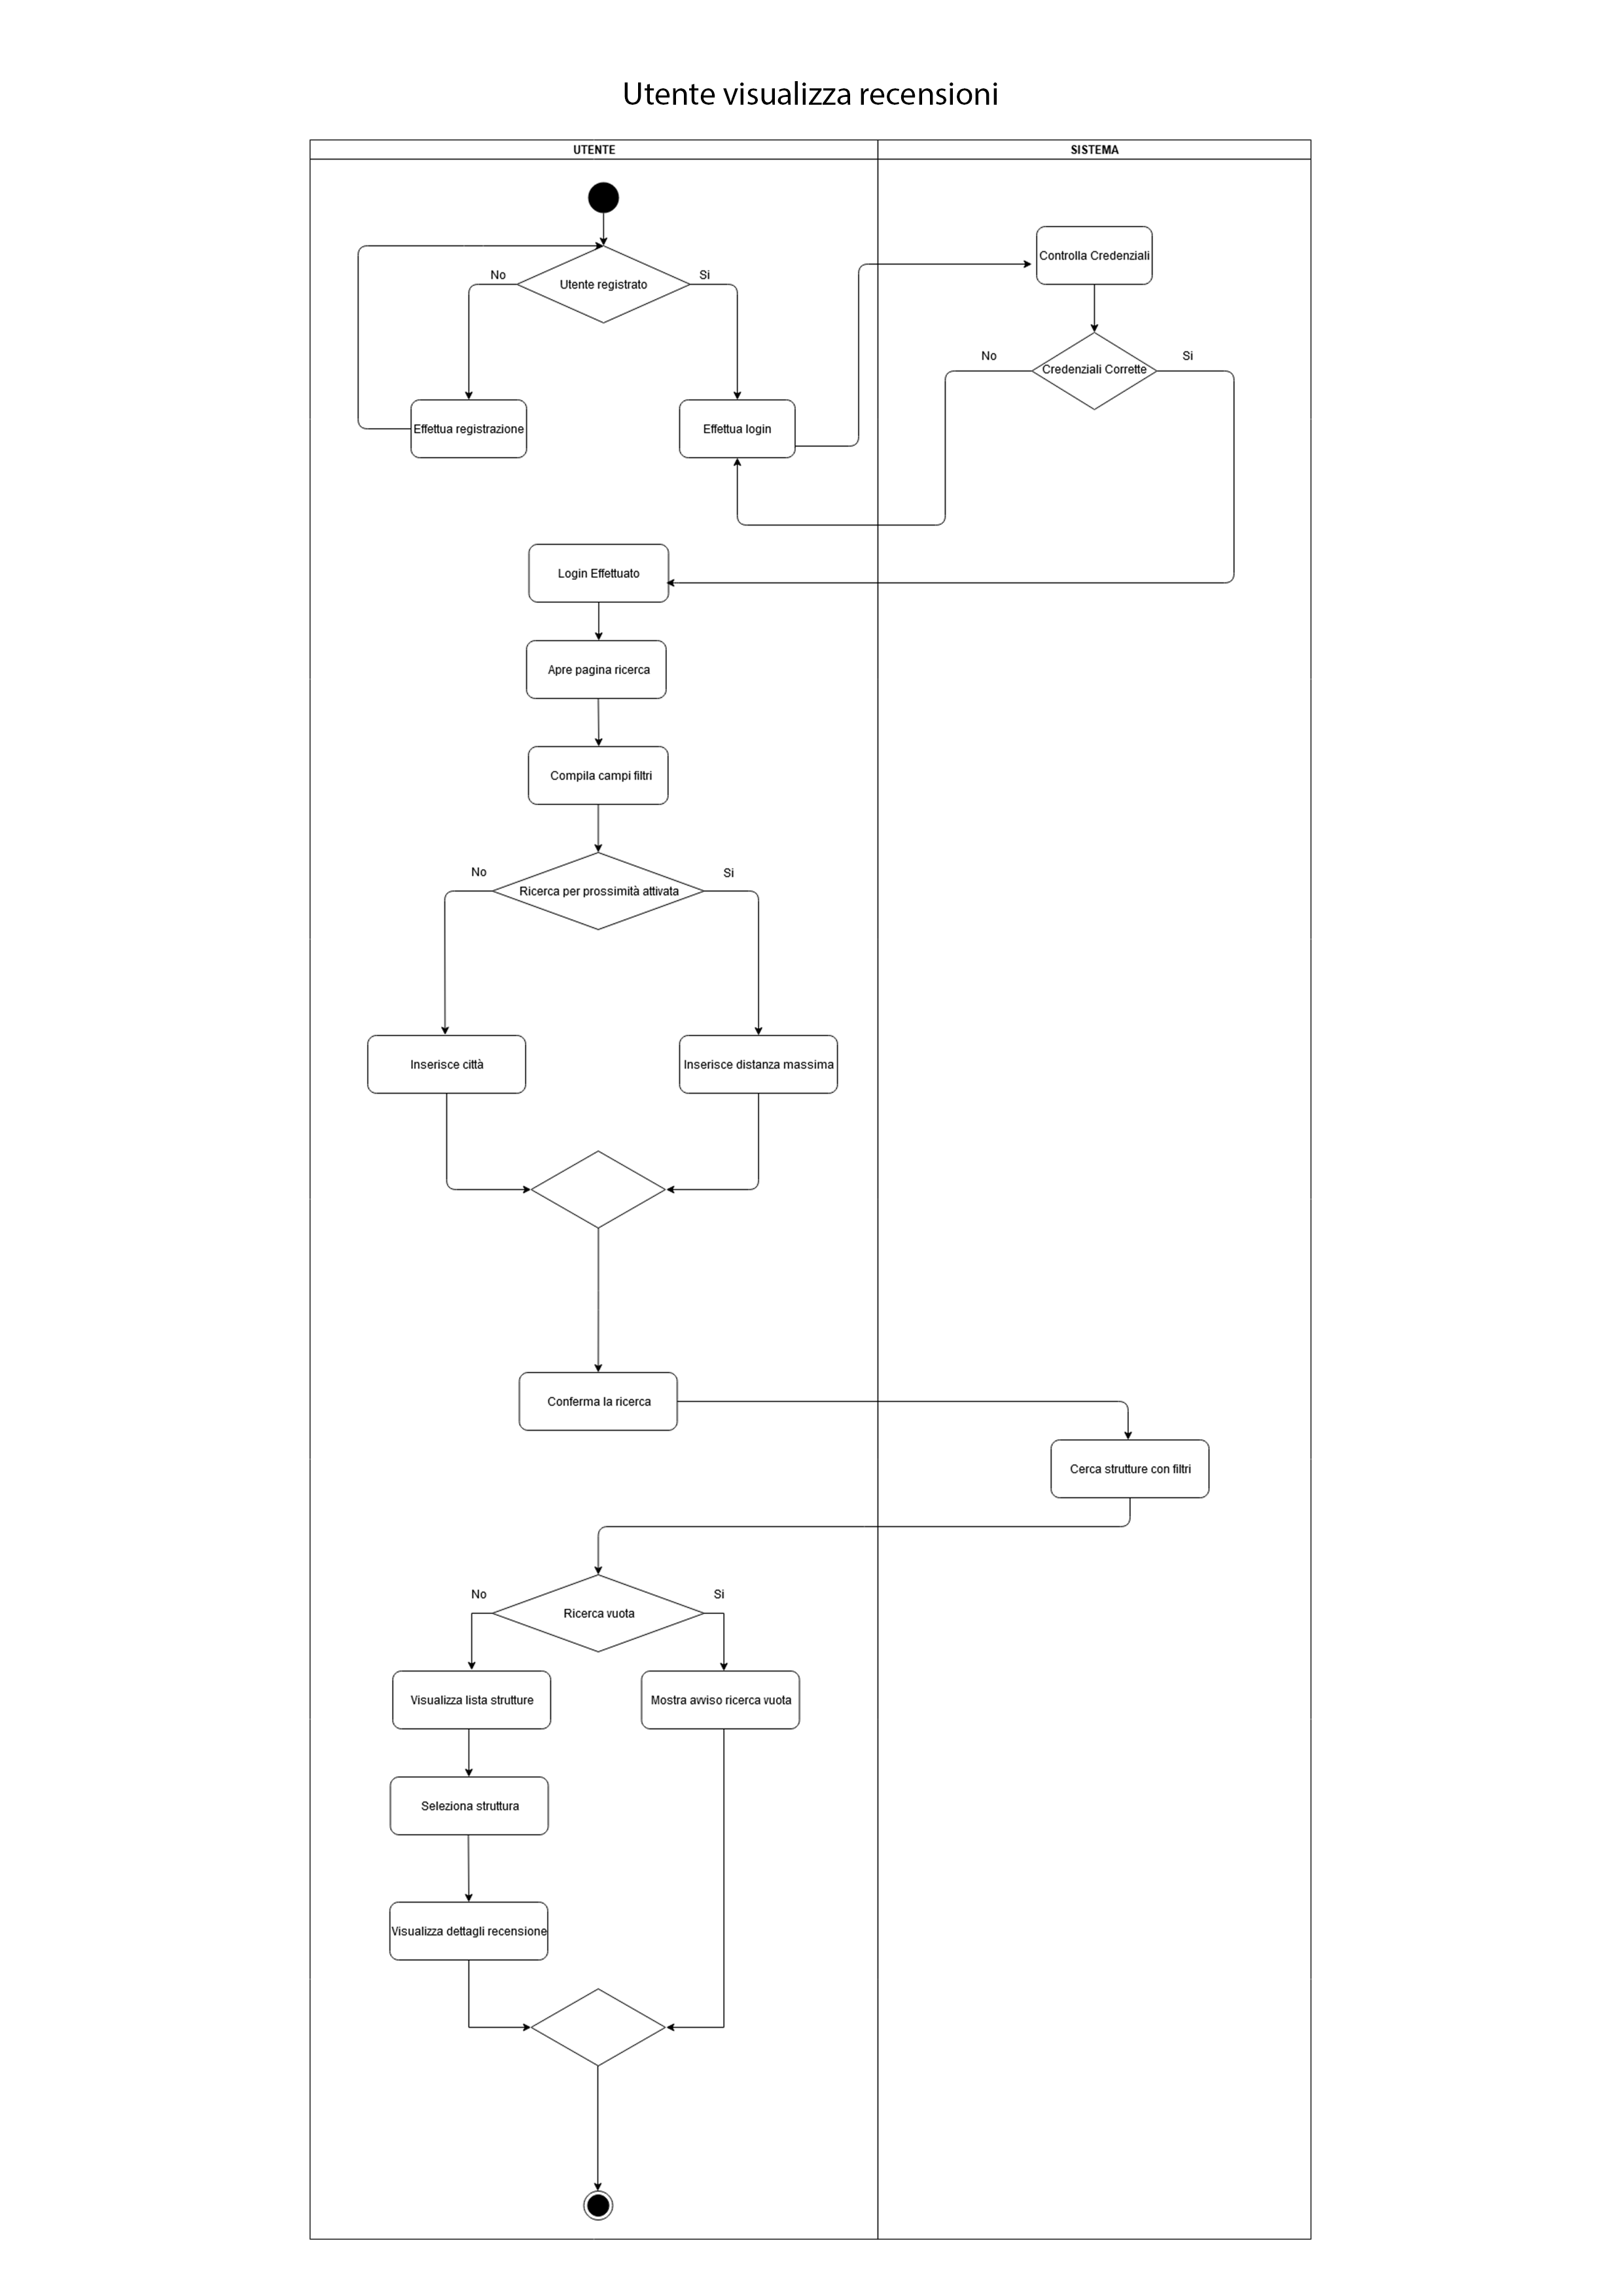
\includegraphics[width=\textwidth]{SequenceAnalisi/11.png}
\end{figure}

%%%%% ===============================================================================
